
\chapter[Mortgage Model]{Mortgage Model}
Transaction costs on property sales are omitted. Add a parameter or variable.

This appendix contains a fairly complete description of the mortgage model with all the equations and figures.

This model is needed to describe bank/buyer behaviour and to calculate the maximum bid that agents make. Mortgage conditions limit the potential bid.

ADD? the discounting equations for the mortgage period"?
sum\_delta, sum\_r?


\subsection{Wealth constraint on m} \label{section-wealth-constraint}

According to the Canada Housing Statistics Program (CHSP), first-time home buyers require a combination of sufficient income and savings in order to enter the housing market. (insert tables? from the CHSP?) We have implemented these facts by making interest rates and mortgage share depend on income and wealth.
We can define individual wealth as:
\[W_i= P_i -M_i  +S_i\]
where 

\begin{tabular}{ll}
$P_i$ & value of owned home\\
$M_i$ & Mortgage on owned home\\
$S_i$ & personal savings = $age*d*W$\\
\end{tabular}

The availability of capital differs for rich and poor. 

The borrowing ratio, $m$ is the fraction of a property's price that can be mortgaged.: $m=M/p_M$. We can develop an expression to capture the relationship between the \gls{borrowing ratio}, $m_i$,  and individual wealth. Figure~\ref{fig-borrowing-ratio} illustrates a plausible mortgage availability  model that is written:

 \[ m_i = 9-\left(\frac{W_i}{\bar W}\right)^{0.1} \]

 
Where $\bar{W}$ is mean wealth and $W_i$ is individual wealth. 
The general relationship is clearly established empirically \cite{}, but location and shape of the curve may vary somewhat. The curve is parameterized, here, so that the bank has a borrowing ratio close to one, perhaps 0.9, since it has many assets. The borrowing ratio for the median wealth holder, perhaps 0.8.


% TODO *** why two axis labels? - and need to label y axis properly

\begin{figure}[htb]
\begin{center}
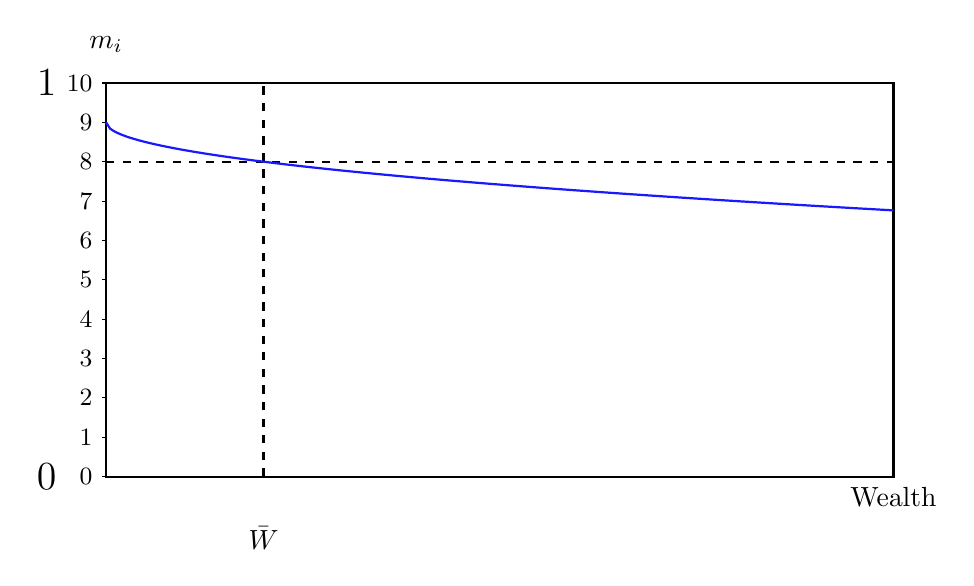
\begin{tikzpicture}[scale=.5]
% \def\bndmax{5}        %https://tex.stackexchange.com/questions/68462/filling-a-complex-region-with-tikz
% \def\bndmin{0.2}
\def\Y{10}  % height of y axis pecent
\def\W{20}  % length  of x axis
\def\Wbar{4}
\def\rbar{8}% this is the prime rate
% Equation   \[ r_i = (A + .5 \frac{\bar{W}}{W_i})\omega\]
% \def\Wmin{.63}  %This sets the lower limit fo the 
\def\Wmin{(\B*\Wbar)/(\Y/\rbar-\A)} %function to keep in in bounds
\tikzset{func/.style={thick,color=blue!90}}	
\draw [thick](\W,\Y)-- (0,\Y)node[left=.5cm]{\Large$1$}node[above=.25cm]{$m_i$} -- (0,0)node[left=.5cm]{\Large$0$}--(\W,0)node[below]{Wealth}--cycle;  	% Axes box
\draw [dashed, thick] (0,\rbar) -- (\W,\rbar);  	% Axes
\draw [thick,dashed] ( \Wbar,0)node[below=.5cm]{$\bar{W}$} -- (\Wbar,\Y);  	% Axes
\foreach \yi in {0,...,\Y} \draw (0,\yi)--(-.1,\yi)node[left]{\small$\yi$};
% \foreach \yi in {0,2,4,6,8,10} \draw (0,\yi)--(-.1,\yi));
% node[left]{\small$\yi$};
% \foreach \yi in {0,2,4,6,8,10}node at (-.1,yi) {{10*yi}} ;
\draw[func,domain=0:\W] plot [samples=200] (\x,(9-\x^.5/2);
\end{tikzpicture}
\end{center}
\caption{Individual borrowing ratio $m_i$ as a function of wealth (in tenths)}
\label{fig-borrowing-ratio}
\end{figure}


\subsubsection{Individualized borrowing rates} \label{section-borowing-rate}

 The cost of capital is known to differ for rich and poor. We tie the individual cost of capital,  $r_i$ for agent $i$, to The lender's target rate $r^{target}$, and to individual wealth. Figure~\ref{fig-capital-cost} illustrates the cost of the borrowing model we implement, which is  roughly consistent  with the stylized facts about lenders. 
 
\begin{equation}
r_i = r^{target}+ K/(W-W_{min}) -K/(\bar W - W_{min})\label{eqn-interest-wealth-relationship}
\end{equation}
%  \begin{equation}. %.  OLD
% r_i = (A + B \frac{\bar{W}}{W_i})\bar r\label{eqn-interest-wealth-relationship}
% \end{equation}

%  Capital cost equation
 
% \[   r^h=\frac{ \delta(1+\dot p  - (1+r)m) \ + \rho   	-\kappa - t } {1-m}    \]

% \begin{figure}[!hb]
% \begin{center}
% 
% Large version
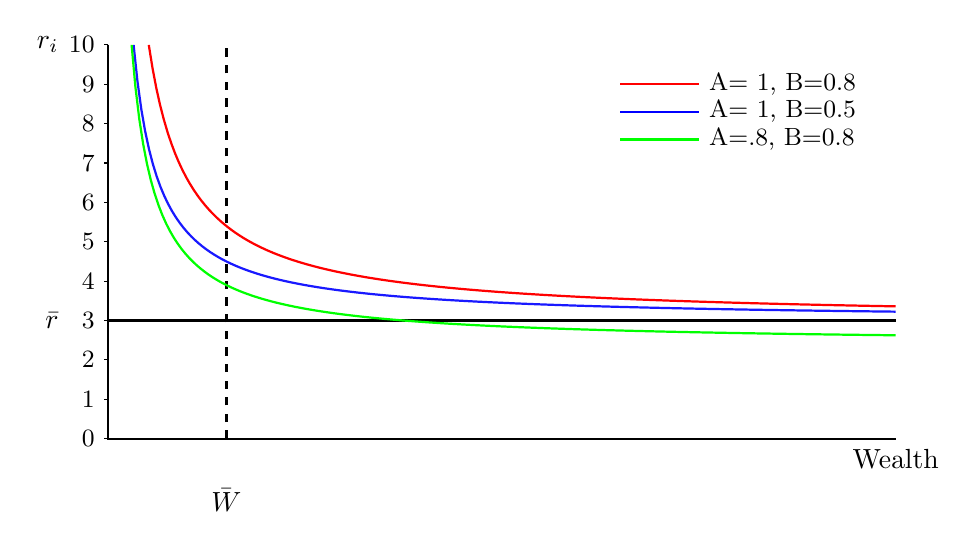
\begin{tikzpicture}[scale=.5]
%\def\bndmax{5}        %https://tex.stackexchange.com/questions/68462/filling-a-complex-region-with-tikz
%\def\bndmin{0.2}
\def \Y {10}  % height of y axis pecent
\def \W {20}  % length  of x axis
\def \Wbar {3} % jmeam wealth
\def \omega {3}
\def \A {1}  %was .5
\def \B {.5}
%Equation   \[ r_i = (A + .5 \frac{\bar{W}}{W_i})\omega\]
\def \Wmin{.63}  %This sets the lower limit fo the 
\def \Wmin{(\B*\Wbar)/(\Y/\omega-\A)} %function to keep in in bounds
	
\tikzset{func/.style={thick,color=blue!90}}	

\draw [thick] (0,\Y)node[left=.5cm]{$r_i$} -- (0,0)--(\W,0)node[below]{Wealth};  	% Axes
\draw [thick] (0,\omega)node[left=.5cm]{$\bar r$} -- (\W,\omega);  	% Axes
\draw [thick,dashed] ( \Wbar,0)node[below=.5cm]{$\bar{W}$} -- (\Wbar,\Y);  	% Axes

\foreach \yi in {0,...,\Y} \draw (0,\yi)--(-.1,\yi)node[left]{\small$\yi$};

\draw[func,domain=\Wmin:\W] plot [samples=200] (\x,{(\A+\B*\Wbar/\x)*\omega});
\def \A {.8}
\draw[func,domain=\Wmin:\W, green] plot [samples=200] (\x,{(\A+\B*\Wbar/\x)*\omega});

\def \A {1}
\def \B {.8}
\draw[func,domain=\Wmin:\W, red] plot [samples=200] (\x,{(\A+\B*\Wbar/\x)*\omega});

\draw [red,  thick](13, 9)--(15,9)node [right, black] {\small A=\ 1,\ B=0.8};
\draw [blue,  thick](13, 8.3)--(15,8.3)node [right, black] {\small A=\ 1,\ B=0.5};
\draw [green, thick](13, 7.6)--(15,7.6)node [right, black] {\small A=.8, B=0.8};
\end{tikzpicture}

% % Small version with equation and parameter values
% \[   r^h=\frac{ \delta(1+\dot p  - (1+r)m) \ + \rho   	-\kappa - t } {1-m}    \]
% \begin{tikzpicture}[scale=.35]
% %\def\bndmax{5}        %https://tex.stackexchange.com/questions/68462/filling-a-complex-region-with-tikz
% %\def\bndmin{0.2}
% \def \Y {10}  % height of y axis percent
% \def \W {18}  % length  of x axis
% \def \Wbar {3} % j mean wealth
% \def \omega {3}
% \def \A {1}  %was .5
% \def \B {.5}
% %Equation   \[ r_i = (A + .5 \frac{\bar{W}}{W_i})\omega\]
% \def \Wmin{.63}  %This sets the lower limit fo the 
% \def \Wmin{(\B*\Wbar)/(\Y/\omega-\A)} %function to keep in in bounds
	
% \tikzset{func/.style={thick,color=blue!90}}	

% \draw [thick] (0,\Y)node[left=.5cm]{$r_i$} -- (0,0)--(\W,0)node[below]{Wealth};  	% Axes
% \draw [thick] (0,\omega)node[left=.5cm]{$\bar r$} -- (\W,\omega);  	% Axes
% \draw [thick,dashed] ( \Wbar,0)node[below=.5cm]{$\bar{W}$} -- (\Wbar,\Y);  	% Axes

% \foreach \yi in {0,...,\Y} \draw (0,\yi)--(-.1,\yi)node[left]{\tiny$\yi$};

% \draw[func,domain=\Wmin:\W] plot [samples=200] (\x,{(\A+\B*\Wbar/\x)*\omega});
% \def \A {.8}
% \draw[func,domain=\Wmin:\W, green] plot [samples=200] (\x,{(\A+\B*\Wbar/\x)*\omega});

% \def \A {1}
% \def \B {.8}
% \draw[func,domain=\Wmin:\W, red] plot [samples=200] (\x,{(\A+\B*\Wbar/\x)*\omega});

% \draw [red,  thick](10, 9)--(12,9)node [right, black] {\tiny A=\ 1,\ B=0.8};
% \draw [blue,  thick](10, 8)--(12,8)node [right, black] {\tiny A=\ 1,\ B=0.5};
% \draw [green, thick](10, 7)--(12,7)node [right, black] {\tiny A=.8, B=0.8};

% \def \W {19}  % length  of x axis
% \node[right] at (\W,9.5){\small$\delta=$discount factor};
% \node[right] at (\W,8.5){\small$\dot p=$appreciation rate};
% \node[right] at (\W,7.5){\small$r=$borrowing rate};
% \node[right] at (\W,6.5){\small$m=$mortgage/price};
% \node[right] at (\W,5.5){\small$\rho=$rental  rate};
% \node[right] at (\W,4.5){\small$\kappa=$op cost rate};
% \node[right] at (\W,3.5){\small$t=$tax rate};
% \node[right] at (\W,2.5){\small$\upsilon=$use value rate};
%  \end{tikzpicture}



% One blue line with x-shift, y-shift
% \begin{figure}
% \begin{tikzpicture}[scale=.5]
% %\def\bndmax{5}        %https://tex.stackexchange.com/questions/68462/filling-a-complex-region-with-tikz
% %\def\bndmin{0.2}
% \def \Y {10}  % height of y axis pecent
% \def \W {20}  % length  of x axis
% \def \Wbar {3} % meam wealth
% \def \rbar {3}% this is the prime rate 

% %\def \Wmin{(\B*\Wbar)/(\Y/\rbar-\A)} %function to keep in in bounds
% \tikzset{func/.style={thick}}	
% 	% Axes
% \draw [thick] (0,\Y)node[left=.5cm]{$r_i$} -- (0,0)--(\W,0)node[below]{Wealth};  
% \foreach \yi in {0,...,\Y} \draw (0,\yi)--(-.1,\yi)node[left]{\small$\yi$};
% \draw [thick] (0,\rbar)node[left=.5cm]{$\bar r$} -- (\W,\rbar);  	% Axes
% \draw [thick,dashed] ( \Wbar,0)node[below=.5cm]{$\bar{W}$} -- (\Wbar,\Y);  	% 

% \def \A {1} %vertical shift aroung \rbar, the prime rate
%  \def \B {1}  % Scales the exponential curveBLUE
%  \def \C {1}  %right shift  
% % \def \Wmin {.4+\B}  %This sets the lower limit fo the 
% \def \Wmin {(\B*\Wbar)/(\Y-\rbar+\A) +\C} %function to keep in in bounds

% \draw[func,domain=\Wmin:\W, color=blue!90] plot [samples=200] (\x,{\rbar-\A+\B*\Wbar/(\x-\C))});
% \node  [align=left, text width =2cm ] at (13, 8.3) {\small y-shift=\A \newline scale=\B \newline x-shift= \C};

%  \end{tikzpicture}
% \caption{Individual borrowing cost as a function of wealth II}
% \label{fig-borrowingrate2}
% \end{figure}

% The rates $\delta,\ \sigma,$ and $r$ depend on the period, $T$. 


% LARGE WITH DIFFERENT PARAMETER VALUES THAN MAOIN FIGURE - MORE SPREAD

% \begin{figure}
% \begin{tikzpicture}[scale=.5]
% %\def\bndmax{5} % https://tex.stackexchange.com/questions/68462/filling-a-complex-region-with-tikz
% %\def\bndmin{0.2}
% \def \Y {10}    % height of y axis as a pecent
% \def \W {20}    % length  of x axis
% \def \Wbar {3}  % mean wealth
% \def \rbar {3}  % the prime rate 

% % Equation   \[ r_i = (A + .5 \frac{\bar{W}}{W_i})\omega\]
% \def \Wmin{.63}  %This sets the lower limit fo the 
% \def \Wmin{(\B*\Wbar)/(\Y/\rbar-\A)} %function to keep in in bounds
% \tikzset{func/.style={thick}}	

% % Axes
% \draw [thick] (0,\Y)node[left=.5cm]{$r_i$} -- (0,0)--(\W,0)node[below]{Wealth};  
% \foreach \yi in {0,...,\Y} \draw (0,\yi)--(-.1,\yi)node[left]{\small$\yi$};
% \draw [thick] (0,\rbar)node[left=.5cm]{$\bar r$} -- (\W,\rbar);  	% Axes
% \draw [thick,dashed] ( \Wbar,0)node[below=.5cm]{$\bar{W}$} -- (\Wbar,\Y);  	% 

% \def \A {1.0}  \def \B {0.5} %BLUE
% \draw[func,domain=\Wmin:\W, color=blue!90] plot [samples=200] (\x,{(\A+\B*\Wbar/\x)*\rbar});
% \draw [ultra thick, color=blue!70 ](13, 8.3)--(15,8.3)node [right, black] {\small A=\A,\ B=\B};

% \def \A {0.5} 
% \def \B {0.5} % GREEN
% \draw[func,domain=\Wmin:\W, color=green] plot [samples=200] (\x,{(\A+\B*\Wbar/\x)*\rbar});
% \draw [thick,  color=green](13, 7.6)--(15,7.6)node [right, black] {\small A=\A, B=\B};

% \def \A {1.0}  \def \B {0.8} % RED
% \draw[func,domain=\Wmin:\W, red] plot [samples=200] (\x,{(\A+\B*\Wbar/\x)*\rbar});
% \draw [thick,  color=red](13, 9)--(15,9)node [right, black] {\small A=\A,\ B=\B};
% % KEY
% \end{tikzpicture}
% \caption{Individual borrowing cost as a function of wealth}
% \label{fig-borrowingrate1}
% \end{figure}
% Figure of cost of borrowing
% \caption[Borrowing cost for agents depending on wealth.]{Borrowing cost for agents depending on wealth, with different values for parameters $A$ and $B$ in Equation~\ref{eqn-interest-wealth-relationship}.} %$A=1$  $B=0.5$ (blue);  $A=1$  $B=0.8$ (red), and  $A=.8$  $B=0.8$ (green).}
% \label{fig-capital-cost}
% \end{center}
% \end{figure}

Where  $r^{target}$ is the bank's target rate of return,  $\bar{W}$ is mean wealth and $W_i$ is individual wealth, $W_{min}$ is the level of wealth the bank requires to lend at all, and $K$ is a parameter for the wealth-sensitivity of lending.\footnote{The median after-tax income of Canadian families and unattached individuals was \$66,800 in 2020 according to Statistics Canada.%'s 
%\href{https://www150.statcan.gc.ca/n1/daily-quotidien/220323/dq220323a-eng.htm}{Canadian Income Survey, 2020}.  \href{https://www150.statcan.gc.ca/t1/tbl1/en/tv.action?pid=1110005501}
% Data released in 2020 by Statistics Canada indicates that t
 The top 1\% of reporting Canadians made, on average, around \$512,000 in a single year \cite{WEB_model-stats-can-canadian-incomes}. % \href{https://www150.statcan.gc.ca/n1/daily-quotidien/201222/dq201222b-eng.htm}{Survey of Financial Security, 2019}.
 %A study by Statistics Canada found that t
 The typical Canadian household now has a median net worth of \$329,900, while the average net worth in Canada is \$738,200 \cite{WEB-model-stats-can-median-net-worth}.  %\href{https://www150.statcan.gc.ca/t1/tbl1/en/tv.action?pid=1110005501}{High income tax filers in Canada}
} The denominator in the last two terms is simply wealth above the lender's minimum. The final term ensures that the target rate is charged for borrowers with average wealth.



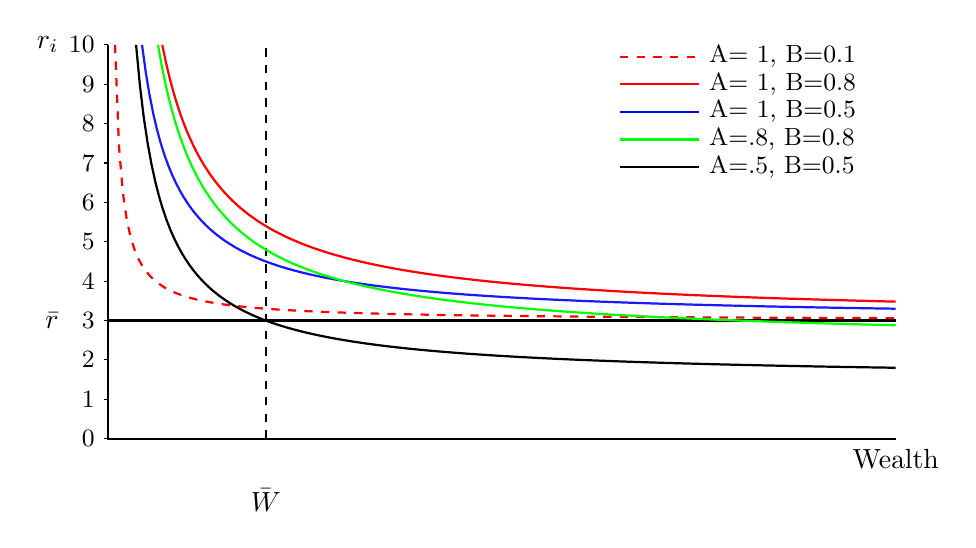
\begin{tikzpicture}[scale=.5]
%\def\bndmax{5}        %https://tex.stackexchange.com/questions/68462/filling-a-complex-region-with-tikz
%\def\bndmin{0.2}
\def \Y {10}  % height of y axis pecent
\def \W {20}  % length  of x axis
\def \Wbar {4} % jmeam wealth
\def \omega {3} % N.B.:  this is r bar

%Equation   \[ r_i = (A + .5 \frac{\bar{W}}{W_i})\omega\]
\def \Wmin{.63}  %This sets the lower limit fo the 
\def \Wmin{(\B*\Wbar)/(\Y/\omega-\A)} %function to keep in in bounds
	
\tikzset{func/.style={thick}}	

\draw [thick] (0,\Y)node[left=.5cm]{$r_i$} -- (0,0)--(\W,0)node[below]{Wealth};  	% Axes
\draw [thick] (0,\omega)node[left=.5cm]{$\bar r$} -- (\W,\omega);  	% Axes
\draw [thick,dashed] ( \Wbar,0)node[below=.5cm]{$\bar{W}$} -- (\Wbar,\Y);  	% Axes

\foreach \yi in {0,...,\Y} \draw (0,\yi)--(-.1,\yi)node[left]{\small$\yi$};

%     ORANGE
% \def \A {1} \def \B {.8}
% \draw[func,domain=\Wmin:\W, orange] plot [samples=200] (\x,{(\A/\x+\B*\X/\Wbar/\x)*\omega});
% \def \A {1} \def \B {.1}
% \draw[func,domain=\Wmin:\W, orange, dashed] plot [samples=200] (\x,{(\A+\B*\X/\Wbar/\x)*\omega});

%     RED
\def \A {1} \def \B {.8}
\draw[func,domain=\Wmin:\W, red] plot [samples=200] (\x,{(\A+\B*\Wbar/\x)*\omega});
\def \A {1} \def \B {.1}
\draw[func,domain=\Wmin:\W, red, dashed] plot [samples=200] (\x,{(\A+\B*\Wbar/\x)*\omega});

%.    BLUE
\def \A {1} \def \B {.5}
\draw[func,domain=\Wmin:\W, blue!90] plot [samples=200] (\x,{(\A+\B*\Wbar/\x)*\omega});
%     GREEN
\def \A {.8} \def \B {.8}
\draw[func,domain=\Wmin:\W, green] plot [samples=200] (\x,{(\A+\B*\Wbar/\x)*\omega});
%.    BLACK
\def \A {.5} \def \B {.5}
\draw[func,domain=\Wmin:\W, black] plot [samples=200] (\x,{(\A+\B*\Wbar/\x)*\omega});


\draw [red,  thick](13, 9)--(15,9)node [right, black] {\small A=\ 1,\ B=0.8};
\draw [red,  thick, dashed](13, 9.7)--(15,9.7)node [right, black] {\small A=\ 1,\ B=0.1};
\draw [blue,  thick](13, 8.3)--(15,8.3)node [right, black] {\small A=\ 1,\ B=0.5};
\draw [green, thick](13, 7.6)--(15,7.6)node [right, black] {\small A=.8, B=0.8};
\draw [black, thick](13, 6.9)--(15,6.9)node [right, black] {\small A=.5, B=0.5};
\end{tikzpicture}


\label{fig-capital-cost}

%The individual cost of capital,  $r_i$ for agent $i$ is tied to a prime rate, $\bar r$ or the bank's target rate, $r^{target}$, and and varies with individual wealth. %Figures~\ref{fig-borrowing-rate1} % and ref{fig-borrowing-rate1} 
%illustratea a  possible  cost-of-borrowing models 

% \begin{align}
%  r_i =  &  \left(A + B \frac{\bar{W}}{W_i}\right) \bar r       \label{eqn-incomeandr1}  \\
%  r_i =  &  \left(\bar r - A + B *\frac{\bar W}{W_i - C}\right) \label{eqn-incomeandr2}  \\
% \end{align}
% Where $\Bar{W}$ is mean wealth and $W_i$ is individual wealth. In Equation~\ref{eqn-incomeandr2},  A determines y-shift, B, the scale, and C the  x-shift for the curve.






 
\subsubsection{Mortgage availability} \label{section-mortgage-availability}
The borrowing of most agents will be constrained. A common rule is that mortgage payments cannot exceed some fraction of disposable income. The wealthy will be able borrow larger amounts and at lower interest rates than the less wealthy.

Many personal finance experts recommend total housing costs account for less than 28\% of \textbf{gross} household income, This gives us an \textbf{income-based  mortgage maximum} of 

\[M^{max}_Yi = \frac{0.28*(\omega+w)}{r_i}\] It is the maximum the bank will let you pay.

We assume $r_i$ is based on the individual's assets, on relative wealth. Where is it calculated for the householder or the bank?

We also have  a \textbf{price-based mortgage maximum} \[M^{max}_P = 0.8P_0\] where $P_0$ is the actual sale price. This is based on the maximum amount of risk that the bank is willing to take on. Combining these conditions, %($P_0$  will not always be the same as the asking price or the warranted price.)

\[M^{max}_Yi = min\left\{\frac{0.28*(\omega+w)}{r_i},  0.8P_0 \right\} \]


% \subsection{The cost of capital}
% The cost of capital is known to differ for rich and poor. This model ties the individual cost of capital,  $r_i$ for agent $i$, to a prime rate, $\bar r$, and to individual wealth. Figure~\ref{fig-borrowing-cost} illustrates the cost of the borrowing model we implement, 
%  \[ r_i = (A + B \frac{\bar{W}}{W_i})\omega\]
% Where $\bar{W}$ is mean wealth and $W_i$ is individual wealth. 

If the expected return on a property is greater than the individual cost of borrowing, it would pay any agent to borrow as much as possible and purchase properties as they can available.\footnote{As pointed out previously,  Equation~\ref{eqn-property-investment-return2} implies a `bang-bang' control - with all sales going to the richest participant unless there are limits on the size of capital flows. For our simulation, we implement such limits. } 
 


\subsubsection{Bank mortgage parameters}

\begin{description}
\item [mortgage period]  mortgage\_period (T)
\item [cost of capital for the bank] r\_prime. The bank's interest rate, $r$, is just the bank rate, (r\_prime) set, for instance, by the Bank of Canada.  
\item [r\_margin] The bank's markup on funds when it lends.  
% \item [r\_target] reference rate that the bank demands on loans on $r^{target}= r^{prime } +r^{margin}$ ? 
\item[lending rate/borrowing rate] The bank lends preferentially to wealthier clients.  
\[r_i=r^{prime} + r^{margin} + \mathrm{individual\_wealth\_adjustment}\] 

\begin{figure}
    \centering
 
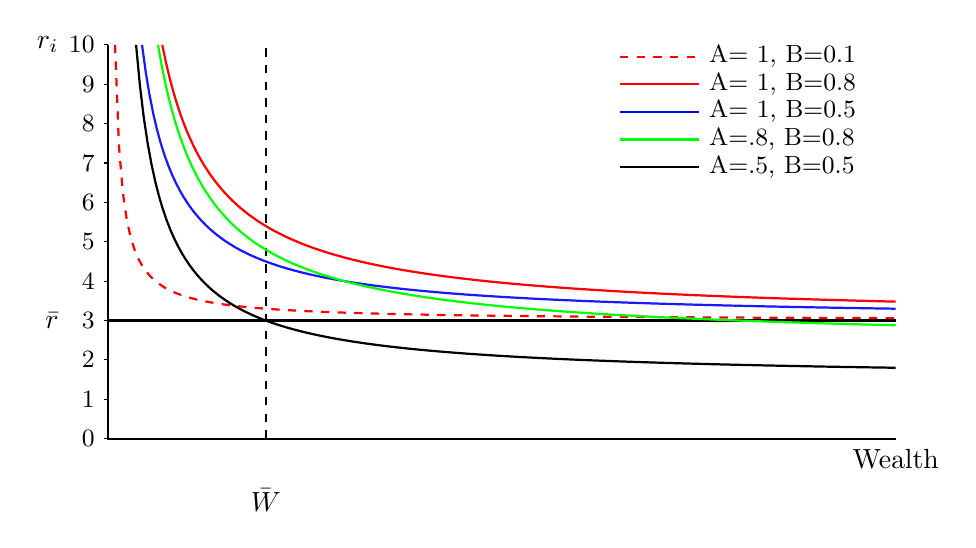
\begin{tikzpicture}[scale=.5]
%\def\bndmax{5}        %https://tex.stackexchange.com/questions/68462/filling-a-complex-region-with-tikz
%\def\bndmin{0.2}
\def \Y {10}  % height of y axis pecent
\def \W {20}  % length  of x axis
\def \Wbar {4} % jmeam wealth
\def \omega {3} % N.B.:  this is r bar

%Equation   \[ r_i = (A + .5 \frac{\bar{W}}{W_i})\omega\]
\def \Wmin{.63}  %This sets the lower limit fo the 
\def \Wmin{(\B*\Wbar)/(\Y/\omega-\A)} %function to keep in in bounds
	
\tikzset{func/.style={thick}}	

\draw [thick] (0,\Y)node[left=.5cm]{$r_i$} -- (0,0)--(\W,0)node[below]{Wealth};  	% Axes
\draw [thick] (0,\omega)node[left=.5cm]{$\bar r$} -- (\W,\omega);  	% Axes
\draw [thick,dashed] ( \Wbar,0)node[below=.5cm]{$\bar{W}$} -- (\Wbar,\Y);  	% Axes

\foreach \yi in {0,...,\Y} \draw (0,\yi)--(-.1,\yi)node[left]{\small$\yi$};

%     ORANGE
% \def \A {1} \def \B {.8}
% \draw[func,domain=\Wmin:\W, orange] plot [samples=200] (\x,{(\A/\x+\B*\X/\Wbar/\x)*\omega});
% \def \A {1} \def \B {.1}
% \draw[func,domain=\Wmin:\W, orange, dashed] plot [samples=200] (\x,{(\A+\B*\X/\Wbar/\x)*\omega});

%     RED
\def \A {1} \def \B {.8}
\draw[func,domain=\Wmin:\W, red] plot [samples=200] (\x,{(\A+\B*\Wbar/\x)*\omega});
\def \A {1} \def \B {.1}
\draw[func,domain=\Wmin:\W, red, dashed] plot [samples=200] (\x,{(\A+\B*\Wbar/\x)*\omega});

%.    BLUE
\def \A {1} \def \B {.5}
\draw[func,domain=\Wmin:\W, blue!90] plot [samples=200] (\x,{(\A+\B*\Wbar/\x)*\omega});
%     GREEN
\def \A {.8} \def \B {.8}
\draw[func,domain=\Wmin:\W, green] plot [samples=200] (\x,{(\A+\B*\Wbar/\x)*\omega});
%.    BLACK
\def \A {.5} \def \B {.5}
\draw[func,domain=\Wmin:\W, black] plot [samples=200] (\x,{(\A+\B*\Wbar/\x)*\omega});


\draw [red,  thick](13, 9)--(15,9)node [right, black] {\small A=\ 1,\ B=0.8};
\draw [red,  thick, dashed](13, 9.7)--(15,9.7)node [right, black] {\small A=\ 1,\ B=0.1};
\draw [blue,  thick](13, 8.3)--(15,8.3)node [right, black] {\small A=\ 1,\ B=0.5};
\draw [green, thick](13, 7.6)--(15,7.6)node [right, black] {\small A=.8, B=0.8};
\draw [black, thick](13, 6.9)--(15,6.9)node [right, black] {\small A=.5, B=0.5};
\end{tikzpicture}


\label{fig-capital-cost}   
    \caption{Individual borrowing rate r\_i}
    \label{fig:Wealth-based}
\end{figure}

 

\item [maximum mortgage share of price] parameter in the calculation of $m_i$. Specific to the functional form used. Set at 0.9. Based on stylized facts from the literature.  No empirical estimates are available. 
\item[wealth sensitivity] of maximum mortgage share of price given total \gls{wealth}, including savings, income and assets. This is a parameter in the calculation of $m_i$. It is specific to functional form used. Set at 0.1. The choice of a function is based on stylized facts from the literature.  No empirical estimates are available.  Used in Equation~\ref{eqn-wealth-based-mortgage}. 

\item [ability to carry a mortgage] 

The share of income that can be used to cover mortgage interest. (rule of thumb: don't spend more than 25\% or 30\% we use 0.28.)
\end{description}
%

\subsection{Maximum mortgage calculation}
The bank puts two  limits on the size of the mortgage, one based on income (a \textbf{carrying constraint}) and one based on wealth (a \textbf{wealth constraint}).

% Mortgage gives 2 numbers. First it pays for a share of the purchase price, second it has an actual maximum. 


\begin{figure}
\centering
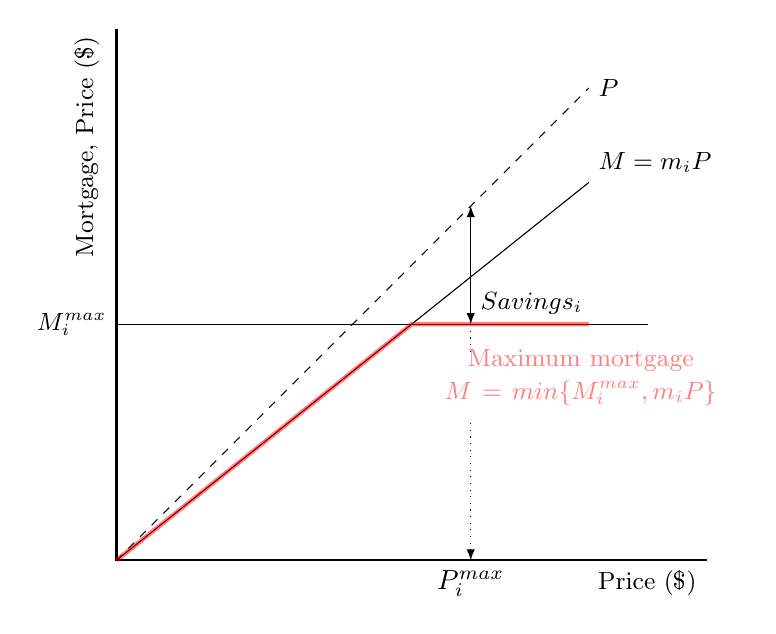
\begin{tikzpicture}	[scale=1.5]
%AXES
\draw[thick] (0,4.5) --(0,0)--(5,0)node[below left]{\small Price (\$)};
\node at (-.25, 3.5)[ rotate=90]{\small Mortgage, Price (\$)};
% M =Mi MAX
\draw[dashed] (0,0)--(4,4)node[right]{\small $P$};
\draw[] (0,2)node[left]{\small $M_i^{max}$}--(4.5,2);%node[right, red]{\small $M = M_i^{max}$};
% M =mi MAX
\draw[] (0,0)--(4,3.2)node[above right]{\small $M = m_iP$};
% COMBINED MAX RED
\draw[ultra thick, red, opacity=.5] (0,0)--(2.5,2)node[below right,  text width=4cm, align = center]{\small \\ Maximum mortgage \\ $M=min\{M_i^{max}, m_iP\}$}--(4.0,2);
% SAVINGS
\draw[latex-latex] (3,2)node[above right] {\small $Savings_i$}--(3,3);
% PMAX
\draw[dotted,latex- ] (3,0)node[below] {$P_i^{max}$}--(3,1.2);
\draw[dotted ] (3,2)--(3,1.72);
\end{tikzpicture}
\caption{The bank's dual mortgage constraint and the savings constraint determine the maximum bid price}
\label{fig:my_label2}
\end{figure}


The two constraints on  mortgage size   that the bank imposes are incorporated in the kinked red line in Figure~\ref{fig:Wealth-based}. The maximum  permitted mortgage  is combined with the savings constraint to determine the maximum price that a potential home buyer can offer.   

% a kink because there are 2 constraints.  The actual mortgage must be below both lines.
The diagonal line, the top dashed diagonal line, is just the price, P = mortgage + savings.
The difference between the two diagonal lines is what the purchaser pays from savings.  
% This is just the constraint. Up to the kink, little $m_i$ is a fraction of price. beyond at little mi becomes a different number - number based on little $m_i$ for everyone
% banks have an advantage since they can practically bid anything
% m - mortgage share
% P - realized price
% M - maximum - 

\begin{figure}
    \centering
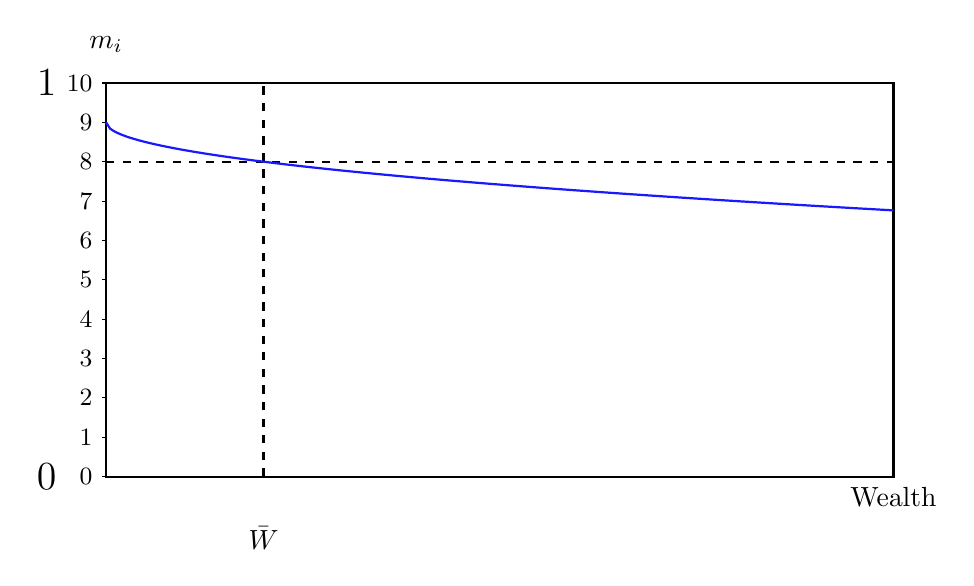
\begin{tikzpicture}[scale=.5]
% \def\bndmax{5}        %https://tex.stackexchange.com/questions/68462/filling-a-complex-region-with-tikz
% \def\bndmin{0.2}
\def\Y{10}  % height of y axis pecent
\def\W{20}  % length  of x axis
\def\Wbar{4}
\def\rbar{8}% this is the prime rate
% Equation   \[ r_i = (A + .5 \frac{\bar{W}}{W_i})\omega\]
% \def\Wmin{.63}  %This sets the lower limit fo the 
\def\Wmin{(\B*\Wbar)/(\Y/\rbar-\A)} %function to keep in in bounds
\tikzset{func/.style={thick,color=blue!90}}	
\draw [thick](\W,\Y)-- (0,\Y)node[left=.5cm]{\Large$1$}node[above=.25cm]{$m_i$} -- (0,0)node[left=.5cm]{\Large$0$}--(\W,0)node[below]{Wealth}--cycle;  	% Axes box
\draw [dashed, thick] (0,\rbar) -- (\W,\rbar);  	% Axes
\draw [thick,dashed] ( \Wbar,0)node[below=.5cm]{$\bar{W}$} -- (\Wbar,\Y);  	% Axes
\foreach \yi in {0,...,\Y} \draw (0,\yi)--(-.1,\yi)node[left]{\small$\yi$};
% \foreach \yi in {0,2,4,6,8,10} \draw (0,\yi)--(-.1,\yi));
% node[left]{\small$\yi$};
% \foreach \yi in {0,2,4,6,8,10}node at (-.1,yi) {{10*yi}} ;
\draw[func,domain=0:\W] plot [samples=200] (\x,(9-\x^.5/2);
\end{tikzpicture}
    \caption{Individual borrowing ratio $m_i$ as a function of wealth}
    \label{fig:Individual-borrowing-rate}
\end{figure}


\textbf{Wealth-based mortgage maximum} 
\begin{align}
m_i^{max\_permitted} = \mathrm{max\_mortgage\_share} - \left(\frac{W_i}{\bar W}\right)^{\mathrm{wealth\_sensitivity}} \label{eqn-wealth-based-mortgage}    
% m_i^{max\_permitted} = 0.9 - \left(\frac{W_i}{\bar W}\right)^{0.1} 
\end{align} 

% **Source**: Ch:model line 580, page 87.. I have done some fiddling Wealth $W_i = P-M+S.  for i - real estate agents estimated price wealth of a property owner as assessed by the bank.
% Where 0.9 is the maximum fraction that can be mortgaged and 0.1 is the wealth sensitivity parameter.

\textbf{Income-based mortgage maximum}

\begin{align}M^{max\_permitted}_i\ = \frac{\mathrm{ability\_to\_carry\_mortgage}*(\omega+\psi+ r_{prime}* \mathrm{savings})}{r_i}\end{align}\label{eqn-income-based-mortgage}
Where ability to carry a mortgage, is the maximum the bank will let an applicant pay based on their wealth.
 
\subsection{Combined mortgage maximum permitted by the bank for new buyers and second home buyers}

The above  two equations specify two constraints on the mortgage,  combining we get:
\begin{align} 
M_i^{max} &= min \left\{ m_i^{max\_permitted}*P, \ M^{max\_permitted}_i \right\} 
% &= min \left\{ \left(0.9- \left( \frac{W_i}{\bar W}\right)^{0.1}\right)P, \  \frac{0.28*(\omega+\psi)}{r_i} \right\}, 
\label{eqn-max-mortgage-combined}
\end{align}

where small $m_i$ a ratio of income, and capital $M_i$ a maximum dollar value.







\section{Maximum bids and reservation price for investors }.\footnote{transaction costs on the sale are omitted. Add a parameter or variable.}
There are two types of investment buyers: institutional buyers and homeowners buying an investment home. They use the same investment formula

We assume that institutional borrowers have no limit on their borrowing capacity ($m_i=1$). home. Existing owners face mortgage constraints form Equation ~\ref{eqn-max-mortgage2} and have different rates $r_i^{target},\ \delta_i$, and $r_i$.

Equation~\ref{eqn-property-investment-return1} gave us the rate of return for a property, rented out. An investor will invest if the expected return on their investment is greater than their target rate of return, % that the investor can price offer for the property and still satisfy
defined by the inequality~\ref{eqn-property-investment-return2}, and equation~\ref{eqn-bid-price}, repeated below, gives the maximum bid price:

\begin{eqnarray}\label{eqn-max-investment-bid}
P_{bank}^{max\_bid} & = \frac{\mathcal{R}_N}{(1-m)r^{target}-\delta \left(1 + \dot P_M^e - (1+r)m\right)} 
\end{eqnarray}
This implies for the bargaining process that if any other potential  has  higher maximum bid, an investor can be eliminated. Combine this observation that each potential bidder will bid up to their maximum bid price, and we know that only the two highest bids matter need be considered.  



\subsubsection{Maximum bid second house buyer}

We assume that existing owners with sufficient savings can bid. They are limited by the limits  that the bank imposes  borrowing capacity.   Purchasing a revenue house is only attractive if the rate return on a rental house exceeds the cost of capital $r_i$. Call this the \textbf{profitability constraint} The maximum bid for this investor is given by Equation~\ref{eqn-max-investment-bid} using one period values for $r_i^{target},\ m_i,\ \delta_i$, and $r_i$.

 \begin{eqnarray}\label{eqn-max-second-bid}
P_{second}^{max\_bid} & = \frac{\mathcal{R}_N}{(1-m_i^{max\_permitted})r_i^{target}-\delta_i \left(1 + \dot P_M^e - (1+r_i)m_i^{max\_permitted}\right)} 
\end{eqnarray}
Notice that this simplifies if any of $r_i^{target},\ \delta_i$, and $r_i$ are set equal. It is possible the cost of capital and the target rate will be the same.

Combining the investment \textbf{profitability constraint} and mortgage constraints

\begin{eqnarray}
P_{second}^{max\_bid} & = min \left\{P_{second}^{max\_bid},\ \frac{\mathrm{savings}_i}{1-m_i^{max\_permitted}},\ \mathrm{saving}s_i + M_i^{max\_permitted}  \right\}  \nonumber
\end{eqnarray}

\subsubsection{Reservation prices for investment owners}
If the current owner of an investment  property gets an high offer higher than their own maximum bid, they will always sell.  


\section{New buyer maximum bids and reservation prices }
A new buyer chooses to move if the income in the city, including the wage amenities exceed the rural income after housing costs, $\psi+A^{Rural}$. 

There are two cases - moving as a buyer and moving as a renter.

\subsection{Moving as a renter}
The gain for a potential renter is 
\begin{align}
gain^{rent}=&net^{city}-net^{Rural}\nonumber\\
=&\left[\psi+\omega-cd+\mathbb{A}^{city}-\mathcal{R}\right]-\left[\psi+\mathbb{A}^{Rural}-a\psi\right] \nonumber\\
=&\ \omega-cd+\mathbb{A}^{net}-\mathcal{R}
\label{eq-move-to-rent}
\end{align}
If rent $\mathcal{R}$ exactly capture housing cost and locational rent, the gain reduces to $\mathbb{A}^{city}-\mathbb{A}^{Rural}$. Normally we would expect property rents to capture this component  as well. 

\subsection{Moving as a buyer}
The gain for a buyer is 
\begin{align}
gain^{buy}=&\ net^{city}-net^{Rural}\nonumber\\
=&\left[\psi+\omega-cd+\mathbb{A}^{city}+(\dot p-r_im_i)P-a\psi\right]-\left[\psi+\mathbb{A}^{Rural}-a\psi\right] \nonumber\\
=&\ \omega-cd+\mathbb{A}^{net}+(\dot p-r_im_i)P  \label{eq-move-to-buy}
\end{align}
This requires that the sum of  locational rent, net amenity and net capital gain be greater than or equal to zero for the in-migrant to buy.

The two decisions  are 
\begin{enumerate}
    \item Move only if $max\{gain^{buy},\ gain^{rent}\} \ge 0$, otherwise do not move to the city.
    
    \item Buy a house if $(\dot p-r_im_i)P\ge  \mathcal{R}$, otherwise rent.
\end{enumerate}

The buyer is subject to the mortgage constraints in Equation~\ref{eqn-max-mortgage-combined}.

We will assume that a first-home buyer always takes the maximum mortgage available to maximize the financial return on the transaction. 

The maximum price a new buyer can bid is also given the bank imposed liquidity constraint is given by Equation~\ref{eqn-max-mortgage-combined}, which we repeat here


\begin{align}
P_i^{max\ bid}= min \left\{\frac{\mathrm{savings}_i}{1-m_i^{max\_permitted}},\  M_i^{max\_permitted} + \mathrm{saving}s_i  \right\}   \nonumber  
\end{align}


\subsection{reservation price for retirees}
Both owners and tenants retire. Homes only become available if they move to the country. 



\subsubsection{Why would a renter move to the country?} 
f the rent is greater than the cost of housing in the country and the lost amenity
\[\mathcal{R} > \ a\psi+ \mathbb{A}^{net}0\]


\subsubsection{Why would an owner move to the country?}
Why would an owner sell a home and move to the country? It would be economically advantageous if the interest on income from the sale exceeds the cost of housing in the country and the lost amenity.
\[r_i(P^{realized}-M) >\ a\psi+ \mathbb{A}^{net}\label{eq:movers-gainA}\]


This value provides a \textbf{reservation price}: 
\[P^{reservation} =\ \frac{a\psi+ \mathbb{A}^{net}}{r_i}+M \label{eq:movers-gainB}\]
This just says that the lowest prices one would sensibly accept is the cost of a house in the country plus enough to cover the mortgage, plus capitalized net amenity.\footnote{transaction costs on the sale are omitted. Add a parameter or variable.}

Should a retiree rent the house out? only if the rent exceeds the  interest on income from the sale:
\[\mathcal{R}^{net}>r_i(P^{realized}-M)\]
This value provides a \textbf{another reservation price}: 
\[P^{reservation} =\ \frac{\mathcal{R}^{net}}{r_i}+M \label{eq:movers-gainC}\]


Sellers should use the investment rule calculated before  do determine a  reservation price in the bargaining process. If they can't get a higher price they  can keep the home as a rental  investment and use the home as collateral for a mortgage on a house in the country.
% For a homeowner, the reservation price is tricky. 
% At this point we only have retirement as a hard boundary to consider. That means that the householder wants to sell in the current period. The gain from moving to the country is 
% \begin{equation}
% Gain=P_{ij}^{expected}-M-\frac{a\psi}{r\_prime} - transaction\ costs - Urban Amenity\  
% \end{equation}\label{eq:movers-gain}
% In the initial model  there are no urban amenities and no transaction costs. We could subtract an urban amenity term, $U_{ij}$ and an transaction cost from equation~\ref{eq:movers-gain}. The amenity term is likely to have little effect, since a buyer will pay extra for the amenity. the transaction cost is actually large and is likely to significantly affect land allocation efficiency.  

The reservation price in in Equation~\ref {eq:movers-gain} is the minimum provides an incentive to sell a home immediately on retiring from the workforce. 



If the sale is delayed by one period, however, the gain is deferred, so the present discounted cost of waiting is, $Gain*\frac{\delta}{1+\delta}$.\footnote{This is simply (1 minus the discount factor) times the deferred amount.} A seller would accept a lower price to avoid this cost of waiting. 

My suggestion is that $\frac{\delta}{1+\delta}P_{ij}^{expected}$ is the \textbf{initial reservation price} for a homeowner on retirement. If the seller does not get this she reduces the reservation price for the next period by (say) 5\% .


\subsubsection{for the Investor-owner}
\textbf{For financial sector in general including those holding investment properties} the problem is easier if anyone offers more than your maximum bid, you should sell the property. 
\begin{eqnarray}
P_{bank}^{reservation} & =    \frac{\mathcal{R}_N}{(1-m)r^{target}-\delta \left(1 + \dot P_M^e - (1+r)m\right)} \label{eqn-res-price-B} \end{eqnarray}

% P_B & \le    \frac{\mathcal{R}_N}{(1-m)r^{target}-\left[ \delta(1+L(P)- (1+r)m\right]}
We call this  $i's$ maximum bid and compute it for all potential buyers and sellers. In each sale the highest $P_B$ will make the purchase. The denominator can be seen as an adjusted rate of return for capitalizing net rents, analogous to the value of $r$ in  the standard capitalization formula. 



\subsubsection{expected price}
So what is the \textbf{expected price}? this should be the expected price from a weighted price regression.\footnote{Wheaton \cite{wheatonVacancySearchPrices1990} suggests ``The combination of price and expected sales time determines the ``expected price'' for a house: market price discounted by expected sales time.'' In his model, vacancy, matching, sales time, and prices with positive vacancy, matching, sales time, and prices are all jointly determined.} Crudely it might be
\[P_{d,t}^e=\beta_1 d + \beta_2 P_{d,t-1} +\epsilon\]
where $\beta_1$ captures spatial correlation and $\beta_2$ captures serial correlation. In this model $\beta_2=1+\dot P$. This simple relationship would tend to change in each period, so the regression would be repeated  at the end of each period  to be used by everyone in the next period. 

You could add $+ \beta_3 (P_{d,t-1}-P_{d,t-2})$ to capture the changing  price change. 



%\textbf{Alternative approaches to the reservation price}

%\begin{eqnarray}
% P_{person}^{reservation} & =   \frac{\mathcal{R}_N}{(1-m)r^{target}-\delta \left(1 + \dot P_M^e - (1+r)m\right)} \label{eqn-res-price-P} \end{eqnarray}


% \begin{tabular}{p{1.5cm}|p{4.5cm}|p{4.5cm}}
%     & reservation & maximum bid\\\hline
% person-buyer    &   & $min \left\{\frac{\mathrm{savings}_i}{1-m_i^{max\_permitted}},\ \mathrm{saving}s_i + M_i^{max\_permitted}  \right\} $ \\\hline
%    person-new  &   & $min \left\{\frac{\mathrm{savings}_i}{1-m_i^{max\_permitted}},\ \mathrm{saving}s_i + M_i^{max\_permitted}  \right\} $ \\\hline
% Bank    &$ min \left\{\frac{\mathrm{savings}_i}{1-m_i^{max\_permitted}},$$\newline$$\mathrm{saving}s_i + M_i^{max\_permitted}  \right\}  $ & \hline
% \end{tabular}

% ALTERNATIVE, NOT USED CALCULATION
%An alternative way to do this, based on old calculations is to compute the realized mortgage share. The realized mortgage $m_i$

%$m_i$ is follows the wealth based rule, $m_i*$ follows the savings based mortgage rule. The realized mortgage share is whichever of these is chosen by the rule in Equation~\ref{eqn-max-mortgage}.

%$m_i^*$, and get the savings.
% We use $m_i$ in calculating the maximum bid for individuals.
%The \textbf{maximum bid} (price that will be offered) is the minimum of $M^{max_i} +S$ and the maximum bid calculated using $m_i$, , (which is calculated independently) if price
% $P\le \frac{M_i^{max}}{m_i}$ 
% and $m_i^*$ if 
% $P\ge \frac{M_i^{max}}{m_i}$, where 
% \[m_i^*=\frac{M_i^{max}}{P}\]

\subsection{Price setting}
\textbf{We have a many-to-many matching problem}. Many buyers and sellers single sellers for each unit. Therefore, for each property that comes on the market each potential seller has a reservation price $P_{ij}^{reservation}$ and there will be a set\footnote{We could allow potential buyers  to approach potential sellers who have not listed with an offer and allow worker-owners to consider retiring early or becoming tenants if an offer is attractive.  This is only likely if speculative pressures are strong. It may require having multiple institutional buyers to make offers more competitive. In that case, initial offers will be closer to the maximum bid price, tending to pull prices up and benefit potential sellers.}  of potential buyers with maximum bids $P_{ij}^{maxbid}$.


This will appear in your data as a set of bids and a reservation price for each property on the market that must be converted to a price for that property using the bargaining rule. The rule is simple: 
\begin{enumerate}
    \item if there is only one maximum bid above the reservation price, split the difference.

    \item If there are two or more maximum bids above the reservation price, the property goes to the highest  and the price is the second highest
\end{enumerate}

\subsubsection{The process}
\begin{enumerate}
\item \textbf{identify the pool of sellers} for each cycle.
    \begin{enumerate}
        \item Agents who a) own and b) age out
        \item Agent  who failed to sell in the previous period.
        \item the bank
    \end{enumerate}
\item \textbf{identify the pool of buyers} 
    \begin{enumerate}
     \item newcomers, 
     \item individuals as investors.
     \item the bank may buy many, (There must be a capital (C) constraint something like $C/\bar P$ to select a number of bank bids in any period.)
    \end{enumerate}

\item \textbf{count buyers and sellers} and use the counts to identify sellers or buyers' market. \# Sellers > \# buyers is a buyers/ market. For a buyer's market  choose the lower price. \footnote{.The is often done with buyers/vacancies. Changes in this ratio are observed to trigger significant movement in rent r market prices.\cite{wheatonVacancySearchPrices1990}. Lisi and Iacobini \cite{lisiEstimatingHousingPrice2015} found  that in the Italian market, ``the difference between the actual selling price and the price obtained in an ideal situation of frictionless housing market – is remarkable. ... the higher the trading frictions on the demand side (more buyers and less sellers), the higher the actual selling price (the price adjustment is positive), whereas the higher the trading frictions on the supply side (less buyers and more sellers), the lower the actual selling price (the price adjustment is negative). '' (they point out that ``Trading frictions are obvious in the housing market, as it takes weeks or months to buy or sell a house (Caplin and Leahy, 2011; Rocheteau and Weill, 2011).'')}  

%a key role is played by the so-called “time-on-the-market (TOM)”. The time it takes to sell a property or “the expected time until the asset is sold when following the optimal policy” (Lippman and McCall, 1986) – commonly known as the TOM – measures the degree of illiquidity of the real estate asset and is a fundamental characteristic differentiating real estate from financial assets. \cite{lisiSearchMatchingProcess2019}
\item \textbf{The pooling problem}  Houses should go at different prices if they have different net rents.  Assume buyers and sellers are indifferent about location (no  local amenities) so only the net rent matters for the ban and only the full rent for individuals.

\item \textbf{Create lists} for the buyer pool and the seller pool. (The bank can appear on the list many times.) 

If the market is efficient, the allocation will maximize the sum or seller and buyer surplus.

\item To select the set of transactors, \textbf{order the lists}. Buyers from highest to lowest, sellers from lowest to highest.

\end{enumerate}


that they are of the same length by dropping the lowest bids or the highest reservation prices. 

\newpage
\textbf{Possibly relevant Example of a matching problem drawn from game theory text}

There are 26  people, some with houses, Each values the house an amount equal to the last three digits of their student numbers. Those on the left of the table don't have a house when the game starts, indicated by a ``0'' in the second column. Those on the right  start with a horse, indicated by a  (1) in the fifth column and half don't. 

\begin{center}
Value and number of houses

\begin{tabular}{|c|c|}
 
\begin{tabular}{lcc}
max bid&start&end  \\ \hline
985  & 0 & 2 \\
829  & 0 & 1 \\
740  & 0 & 1 \\
650  & 0 & 1 \\
643  & 0 & 1 \\
611  & 0 & 1 \\\hline
532  & 0 & \color{red}1  \\
356  & 0 & \color{red} 1   \\
270  & 0 & \color{red} 1  \\
135  & 0 & 0    \\%69 & 1  & 0
   
\end{tabular}

&
\begin{tabular}{lcc}
reservation&start&end \\ \hline
 50 & 1  & 0 \\
127 & 1  & 0 \\
190 & 1  & 0  \\
245 & 1  & 0 \\
 324 & 1  & 0 \\
 522 & 1 & \color{red} 1\\\hline
 738 & 1  &  \color{blue}0 \\
 829 &1  &  \color{blue}0 \\
832 & 1 & \color{blue}0\\
   &  &              \\%69 & 1  & 0 
\end{tabular}

\end{tabular}
\end{center}


 
  \begin{tikzpicture}[scale=.8]
%  \draw [gray, opacity=.7]
 (0,0) grid (7,7);
\draw [<->] (0,10.5) node[above]{value}-- (0,0) -- (10,0) node[below]{Houses};

\draw [red, thick] (0,9.85)node[above right]{985}--(1,9.85)--(1,8.29 )node[above right]{829}--(2,8.29 )--(2,7.40 )node[above right]{740}--(3,7.40 )--(3,6.50 )node[above right]{350}--(4,6.50 )--(4,6.43)node[above right]{643}--(5,6.43)--(5,6.11)node[above right]{611}--(6,6.11)--(6,5.32)node[above right]{532}--(7,5.32)--(7,3.56)node[above right]{356}--(8,3.56)--(8,2.70)node[above right]{270}--(9,2.70)--(9,1.35)node[left]{DEMAND}node[above right]{135}--(10,1.35); 

\draw [blue, thick] (0,.50)node[above right]{50}--(1,.5)--(1,1.27 )node[above right]{127}--(2,1.27 )--(2,1.90 )node[above right]{190}--(3,1.90 )--(3,2.45 )node[above right]{245}--(4,2.45 )--(4,3.24)node[above right]{324}--(5,3.24)--(5,5.22)node[above right]{522}--(6,5.22)--(6,7.38)node[above right]{738}--(7,7.38)--(7,8.29)node[above right]{829}--(8,8.29)--(8,8.32)node[above right]{832}--(9,8.32)node[right]{SUPPLY}; 
%,2.5) ;
%\draw [blue, dashed] (0,4.5) node[left]{large bill}--(8.33, 4.5)-- (8.33,0)node[below] {large user Q};
%\draw [green, dashed] (0,0) --(8.33, 4.5);
%\draw [green, dashed] (0,0) --(1.66, 2.5);

%\draw [<->, shift={(7 cm,0)}] (0,6) -- (0,0) -- (5,0);
\end {tikzpicture}

The gain for any person is the difference between the transaction price  for a house and the amount they value a house




At the same time, for each p. NOT. DONE
\begin{eqnarray}
P_{bank}^{reservation} & \le  P_{person}^{max\_bid} \end{eqnarray}


\begin{lstlisting}
# parameters - max interest payment 
max_mortgage_share = 0.28 # ability to cover a mortgage

# Max mortgage

wealth = property_value - mortgage + savings
mean_weath = sum(wealth)/number_of_people

def get_max_mortgage(self, applicant):
    max_mortgage =  ...
    
    return max_mortgage
\end{lstlisting}





\newpage\hrule
\section{TABLE OF BID AND RESERVATION PRICES}
\hrule




\section{For investors}
 Institutional borrowers have no limit on their borrowing capacity ($m_i=1$). home. Existing owners face mortgage constraints .
maximum bid price:\footnote{transaction costs on the sale are omitted. Add a parameter or variable.}

\begin{eqnarray}\label{eqn-max-investment-bid}
P_{bank}^{max\_bid} & = \frac{\mathcal{R}_N}{(1-m)r^{target}-\delta \left(1 + \dot P_M^e - (1+r)m\right)} 
\end{eqnarray}


\subsubsection{Maximum bid second house buyer}

 \begin{eqnarray}\label{eqn-max-second-bid}
P_{second}^{max\_bid} & = \frac{\mathcal{R}_N}{(1-m_i^{max\_permitted})r_i^{target}-\delta_i \left(1 + \dot P_M^e - (1+r_i)m_i^{max\_permitted}\right)}  \nonumber
\end{eqnarray}

Combining the investment \textbf{profitability constraint} and mortgage constraints

\begin{eqnarray}
P_{second}^{max\_bid} & = min \left\{P_{second}^{max\_bid},\ \frac{\mathrm{savings}_i}{1-m_i^{max\_permitted}},\ \mathrm{saving}s_i + M_i^{max\_permitted}  \right\}  \nonumber
\end{eqnarray}

\subsubsection{Reservation prices for investment owners}
 if anyone offers more than your maximum bid, you should sell the property. 
\begin{eqnarray}
P_{investor}^{reservation} & =    \frac{\mathcal{R}_N}{(1-m)r^{target}-\delta \left(1 + \dot P_M^e - (1+r)m\right)}  \nonumber\end{eqnarray}


\section{For new buyers}

There are two cases - moving as a buyer and moving as a renter.

\subsection{Moving to the city and renting}
The gain for a potential renter is 
\begin{align}
gain^{rent}
=&\ \omega-cd+\mathbb{A}^{net}-\mathcal{R}
  \nonumber
\end{align}

\subsection{Moving to the city and  buying}
The gain for a buyer is 
\begin{align}
gain^{buy}=&\ \omega-cd+\mathbb{A}^{net}+(\dot p-r_im_i)P   \nonumber
\end{align}
\textbf{The rule to apply}
\begin{enumerate}
    \item \textbf{Move} only if $max\{gain^{buy},\ gain^{rent}\} \ge 0$, otherwise do not move to the city.
    
    \item \textbf{Buy} a house if $(\dot p-r_im_i)P\ge  \mathcal{R}$, otherwise rent.
\end{enumerate}
\textbf{Maximum bid for new  resident}
\begin{align}
P_i^{max\ bid}= min \left\{\frac{\mathrm{savings}_i}{1-m_i^{max\_permitted}},\  M_i^{max\_permitted} + \mathrm{saving}s_i  \right\}   \nonumber  
\end{align}


\section{Behaviour of  retirees}
Both owners and tenants retire. Homes only become available if they move to the country. 
\subsubsection{A renter move to the country if} 
\[\mathcal{R} > \ a\psi+ \mathbb{A}^{net}0\]
\subsubsection{An owner sells and moves to the country if}
\[r_i(P^{realized}-M) >\ a\psi+ \mathbb{A}^{net}\] \subsection{ Combined owner reservation price}: 
\[P_{owner-sell}^{reservation} =\ \frac{a\psi+ \mathbb{A}^{net}}{r_i}+M \]

\subsubsection{An owner Rents and moves to the country if} 
\[\mathcal{R}^{net}>r_i(P^{realized}-M)\]
This value provides a \textbf{another reservation price}: 
\[P_{owner-rent}^{reservation} =\ \frac{\mathcal{R}^{net}}{r_i}+M \]

\subsubsection{Retiring owner's reservation price}
\[P_{owner-combined}^{reservation}= max\left\{ P_{owner-sell}^{reservation} ,\ P_{owner-rent}^{reservation}\right\}\]

\hrule

